\documentclass{bmstu}[a4paper]

\renewcommand\labelitemi{--}


\usepackage{threeparttable}

\bibliography{biblio}

\begin{document}
	
	\makereporttitle
	{Информатика и системы управления} % Название факультета
	{Программное обеспечение ЭВМ и информационные технологии} % Название кафедры
	{лабораторной работе №~4} % Название работы (в дат. падеже)
	{Анализ алгоритмов} % Название курса (необязательный аргумент)
	{Параллельные вычисления на основе нативных потоков} % Тема работы
	{} % Номер варианта (необязательный аргумент)
	{Савинова~М~Г./ИУ7-51Б} % Номер группы/ФИО студента (если авторов несколько, их необходимо разделить запятой)
	{Волкова~Л.~Л.} % ФИО преподавателя
	
	\maketableofcontents
	
	\chapter*{Введение}
\addcontentsline{toc}{chapter}{Введение}

\textbf{Расстояние Левенштейна}~--- это метрика, используемая для измерения разницы между двумя строками. Она вычисляет минимальное количество односимвольных изменений (вставок, удалений или замен), необходимых для преобразования одной строки в другую.

Расстояние Левенштейна обычно используется в различных областях~\cite{analysis-lev-damlev}, в том числе:
\begin{enumerate}
    \item \textbf{Проверка орфографии:} выявление и исправление ошибок для слов на основе их расстояния Левенштейна.
    \item \textbf{Анализ последовательности ДНК:} измерение сходства между последовательностями ДНК позволяет исследователям сравнивать и анализировать генетические данные.
    \item \textbf{Обработка естественного языка (НЛП):} используется в таких задачах, как классификация текстов, поиск информации и машинный перевод, для определения сходства между текстами.
\end{enumerate}

\textbf{Расстояние Дамерау\,--\,Левенштейна} является расширением расстояния Левенштейна, которое не учитывает транспозиции. Дополнительная операция позволяет обрабатывать случаи, когда символы меняются местами или переупорядочиваются.

\textbf{Целью} данной лабораторной работы является изучение, реализация и исследование алгоритмов поиска расстояний Левенштейна и Дамерау\,--\,Левенштейна.

Необходимо выполнить следующие \textbf{задачи}:
\begin{enumerate}[label={\arabic*)}]
    \item изучить алгоритмы Левенштейна и Дамерау\,--\,Левенштейна для нахождения редакционного расстояния между строками;
    \item реализовать данные алгоритмы;
    \item выполненить сравнительный анализ алгоритмов по затрачиваемым ресурсам (времени, памяти);
    \item описать и обосновать полученные результаты в отчете.
\end{enumerate}
	\chapter{Аналитическая часть}
\section{Расстояние Левенштейна}

\textbf{Расстояние Левенштейна}~--- это минимальное количество редакторских операций вставки, замены и удаления, которые необходимо выполнить для преобразования одной строки в другую~\cite{levenshtein}. 

Каждая операция имеет свою цену($w$). Редакционное предписание~--- это последовательность операций с сумарной минимальной стоимостью, которую необходимо выполнить для получения из первой строки вторую. Эта цена и есть искомое расстояние Левенштейна.

Введем следующие обозначения:
\begin{enumerate}[label=\arabic*)]
    \item \textbf{I}~(от англ. insert)~--- вставка ($w(\lambda, b) = 1$);
    \item \textbf{R}~(от англ. replace)~--- замена ($w(a, b) = 1$, $a \neq b$);
    \item \textbf{D}~(от англ. delete)~--- удаление ($w(a, \lambda) = 1$).
\end{enumerate}

Также рассмотрим функцию $D(i, j)$: ее значением является
редакционное расстояние между строками $S_1[1...i]$ и $S_2[1...j]$.

Расстояние Левенштейна между двумя строками $S_{1}$ и $S_{2}$ (длиной $M$ и $N$ соответственно) рассчитывается по следующей рекуррентной формуле:
\begin{equation}
	\label{eq:L}
	D(i, j) =
	\begin{cases}
		0, &\text{i = 0, j = 0}\\
		i, &\text{j = 0, i > 0}\\
		j, &\text{i = 0, j > 0}\\
		min \begin{cases}
			D(i, j - 1) + 1,\\
			D(i - 1, j) + 1,\\
			D(i - 1, j - 1) +  m(S_{1}[i], S_{2}[j]), \\
		\end{cases}
		&\text{i > 0, j > 0}
	\end{cases}
\end{equation}
где сравнение символов строк $S_1$ и $S_2$ рассчитывается таким образом:
\begin{equation}
	\label{eq:m}
	m(a, b) = \begin{cases}
		0 &\text{если a = b,}\\
		1 &\text{иначе.}
	\end{cases}
\end{equation}

\section{Расстояние Дамерау~---~Левенштейна}

\textbf{Расстояние Дамерау~---~Левенштейна}~--- это мера разницы двух строк, определяемая как минимальное количество операций вставки, удаления, замены и транспозиции (перестановки двух соседних символов), необходимых для перевода одной строки в другую~\cite{analysis-lev-damlev}. Является расширением расстояния Левенштейна, поскольку помимо трех базовых операций содержит еще операцию транспозиции $T$ (от англ. transposition).

Расстояние Дамерау~---~Левенштейна определятся следующей рекуррентной формуле:

\begin{multline}
    D(m, n) =\\ =
    \begin{cases}
        0, &\text{i = 0, j = 0}\\
        i, &\text{j = 0, i > 0}\\
        j, &\text{i = 0, j > 0}\\
        \min
        \begin{cases}
            D(i, j - 1) + 1,\\
            D(i - 1, j) + 1,\\
            D(i - 1, j - 1),\\
            D(i - 2, j - 2) + 1,
        \end{cases} 
        &\begin{aligned}
            & \text{если $i, j > 1$}, \\
            & S_{1}[i] = S_{2}[j - 1], \\
            & S_{1}[i - 1] = S_{2}[j],
        \end{aligned} \\
        \min
        \begin{cases}
            D(i - 1, j) + 1, \\
            D(i, j - 1) + 1, \\
            D(i - 1, j - 1) + \text{m}(S_1[i], S_2[j])
        \end{cases} &\text{иначе.}
    \end{cases}
    \label{eqn:recur-damlev}
\end{multline}

\section*{Вывод}
В данном разделе были рассмотрены алгоритмы нахождения расстояния Левенштейна и Дамерау~---~Левенштейна.
Формулы для вычисления этих расстояний задаются \textbf{рекуррентно}, поэтому алгоритмы для нахождения их расстояний можно реализовать как \textit{итеративно}, так и \textit{рекурсивно}.

	\chapter{Конструкторская часть}
В данной части работы будут рассмотрены схемы алгоритмов различных реализаций сортировки слиянием.

\section{Требования к программному обеспечению}

К программе предъявлены ряд требований:

\begin{itemize}
	\item возможность выбора действий;
	\item работа с массивами и <<нативными>> потоками.
\end{itemize}

\section{Требования к временным замерам}
\textbf{Процессорное время}~--- это время, которое потратил процессор  на выполнение задачи.

\textbf{Реальное время}~--- время, прошедшее с начала выполнения задачи \cite{time}. 

В данной работе, при использовании многопоточности возможно
ожидание одними потоками выполнения других потоков. Поток не выполняет
никаких действий в это время, поэтому простой не влияет на процессорное время, однако это влияет на результирующее реальное время, поэтому для корректного сравнения различных реализаций  по времени работы стоит замерять и сравнивать реальное время
выполнения реализаций алгоритмов.

\section{Схемы алгоритмов}

На рисунках \ref{img:mergeSort}--\ref{img:merge} приведены схемы алгоритмов различных вариаций алгоритма сортировки слиянием

\includeimage
{mergeSort} % Имя файла без расширения (файл должен быть расположен в директории inc/img/)
{f} % Обтекание (без обтекания)
{H} % Положение рисунка (см. figure из пакета float)
{1\textwidth} % Ширина рисунка
{Схема алгоритма сортировки слиянием, при использовании 1 потока} % Подпись рисунка

\includeimage
{mergeSortMultiThread} % Имя файла без расширения (файл должен быть расположен в директории inc/img/)
{f} % Обтекание (без обтекания)
{H} % Положение рисунка (см. figure из пакета float)
{1\textwidth} % Ширина рисунка
{Схема алгоритма сортировки слиянием, при использовании нескольких потоков} % Подпись рисунка

\includeimage
{merge} % Имя файла без расширения (файл должен быть расположен в директории inc/img/)
{f} % Обтекание (без обтекания)
{H} % Положение рисунка (см. figure из пакета float)
{0.9\textwidth} % Ширина рисунка
{Схема алгоритма слияния отсортированных последовательностей} % Подпись рисунка

\newpage

Алгоритм слияния отсортированных последовательностей используется во всех рассматриваемых версиях алгоритма, в случае использования нескольких потоков, слияние будет происходить в отдельном потоке.

При использовании нескольких потоков (схема на рис.~\ref{img:mergeSortMultiThread}), число доступных потоков делится на 2 при каждом шаге рекурсии, в таком случае число доступных потоков поровну разделяется при каждом разбиении массива на подмассивы для слияния.

\section*{Вывод}
В данном разделе  были построены схемы рассматриваемых алгоритмов.


	\chapter{Технологический раздел}

В данной части работы будут описаны средства реализации программы, а также листинги и  модульные  тесты.
	
\section{Средства реализации}
Алгоритмы для данной лабораторной работы были реализованы на языке C++, так как в библиотеке приведенного языка присутствует функция \texttt{clock}, которая  позволяет получить количество тиков с времени начала выполнения программы, при делении полученного значения на макропеременную \texttt{CLOCKS\_PER\_SEC}, возможно получение значения времени в секундах~\cite{cpp-time}.

Для создания потоков и работы с ними был использован класс \texttt{thread} из стандартной библиотеки выбранного языка~\cite{std-thread}.

В листинге \ref{lst:thead-example.cpp}, приведен работы с описанным классом, каждый объект класса представляет собой поток операционной системы, что позволяет нескольким функциям выполняться параллельно~\cite{std-thread}. 
\includelistingpretty
{thead-example.cpp} % Имя файла с расширением (файл должен быть расположен в директории inc/lst/)
{c++} % Язык программирования (необязательный аргумент)
{Пример работы с классом thread} % Подпись листинга

Поток начинает свою работу после создания объекта, соответствующего класса, запуская функцию, приведенную в его конструкторе~\cite{std-thread}.
В данном примере будет запущен 1 поток, который выполнит функцию \texttt{foo},
которая выведет число 10 на экран.

\section{Реализация алгоритмов}
Листинги~\ref{lst:merge.cpp}--\ref{lst:mergeSortMultiThread.cpp} исходных кодов программ приведены в приложении. 

\section{Тестирование}

В таблице \ref{t:mod_tests} приведены модульные  тесты для разработанных алгоритмов сортировки. Все приведенные массивы были отсортированы с помощью сортировки слиянием, в столбце <<Один поток>>
показаны результаты использования реализации с 1 потоком,  в столбце <<Несколько потоков>> показаны результаты использования реализации с несколькими потоками. Все тесты пройдены успешно.
\begin{table}[ht]
	\small
	\begin{center}
		\begin{threeparttable}
			\caption{Модульные тесты}
			\label{t:mod_tests}
			\begin{tabular}{|c|c|c|c|c|}
				\hline
				\bfseries Массив
				& \bfseries Размер
				& \bfseries Ожидаемый р-т
				& \multicolumn{2}{c|}{\bfseries Фактический результат} \\ \cline{4-5}
				& & & \bfseries Один поток & \bfseries  Несколько потоков \\
				\hline
				1 2 3 4  & 4 & 1 2 3 4 & 1 2 3 4 & 1 2 3 4 \\
				\hline
				4 3 2 1 & 4 & 4 3 2 1 & 4 3 2 1 & 4 3 2 1 \\
				\hline
				3 5 1 6 & 4 & 1 3 5 6  & 1 3 5 6 & 1 3 5 6 \\
				\hline
				-5 -1 -3 -4 -2 & 5 & -5 -4 -3 -2 -1 & -5 -4 -3 -2 -1 & -5 -4 -3 -2 -1 \\
				\hline
				1 -3 2 9 -9 & 5 & -9 -3 1 2 9  & -9 -3 1 2 91 & -9 -3 1 2 9 \\
				\hline
			\end{tabular}	
		\end{threeparttable}	
	\end{center}
\end{table}


\textbf{Вывод}
 В данной части работы были представлены листинги реализованных алгоритмов и тесты, успешно пройденные программой.

	\chapter{Исследовательская часть}

\section{Технические характеристики}
Технические характеристики устройства, на котором выполнялись замеры по времени, представлены далее.
\begin{itemize}
	\item Процессор: AMD Ryzen 5 5500U\,--\,2.10 ГГц;
	\item Оперативная память: 16 ГБайт;
	\item Операционная система: Windows 10 Pro 64-разрядная система версии 22H2.
\end{itemize}

При замерах времени ноутбук был включен в сеть электропитания и был нагружен только системными приложениями.

\section{Демонстрация работы программы}
На рисунке \ref{img:demonstration} представлена демонстрация работы разработанного ПО.  
\begin{figure}[h]
	\centering
	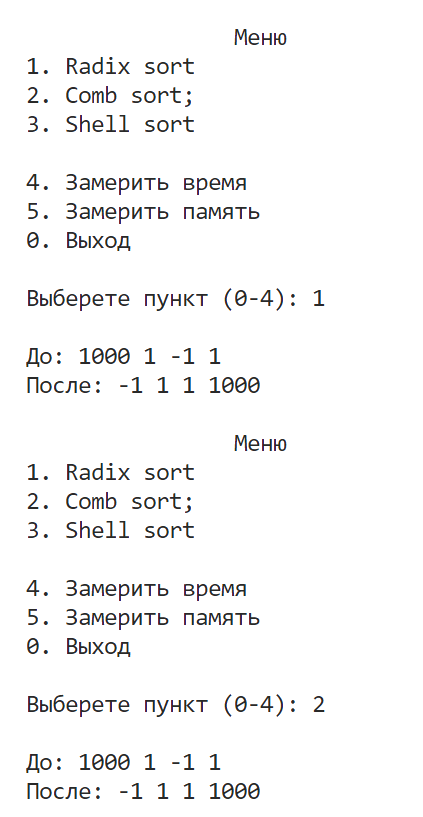
\includegraphics[height=0.3\textheight]{img/prog_work.png}
	\caption{Демонстрация работы программы}
	\label{img:demonstration}
\end{figure}

\section{Временные характеристики}
Все замеры проводились на квадратных матрицах. Поскольку замеры по времени имеют некоторую погрешность, замеры производились 100 раз, а затем вычислялось среднее арифметическое значение.

Результаты замеров приведены в таблицах \ref{tbl:time_even}--\ref{tbl:time_odd}.

На рисунках \ref{plt:time_01}--\ref{plt:time_02} приведены графики зависимостей работы алгоритмов от размеров матриц.

\begin{table}[h!]
    \caption{Результаты замеров времени (четные размеры матрицы)}
    \label{tbl:time_even}
	\centering
		\begin{tabular}{||c|c|c|c||}
			\hline
			& \multicolumn{3}{c|}{Время, мкс} \\ \cline{2-4}
			Размер матрицы & Стандартный & Виноград & (опт.) Виноград
			\csvreader{tables/time_even.csv}{}
			{\\\hline \csvcoli & \csvcolii & \csvcoliii & \csvcoliv} 
			\\
			\hline
		\end{tabular}
\end{table}

\begin{table}[h!]
    \caption{Результаты замеров времени (нечетные размеры матрицы)}
    \label{tbl:time_odd}
	\centering
		\begin{tabular}{||c|c|c|c||}
			\hline
			& \multicolumn{3}{c|}{Время, мкс} \\ \cline{2-4}
			Размер матрицы & Стандартный & Виноград & (опт.) Виноград
			\csvreader{tables/time_odd.csv}{}
			{\\\hline \csvcoli & \csvcolii & \csvcoliii & \csvcoliv} 
			\\
			\hline
		\end{tabular}
\end{table}

\begin{figure}[H]
	\centering
	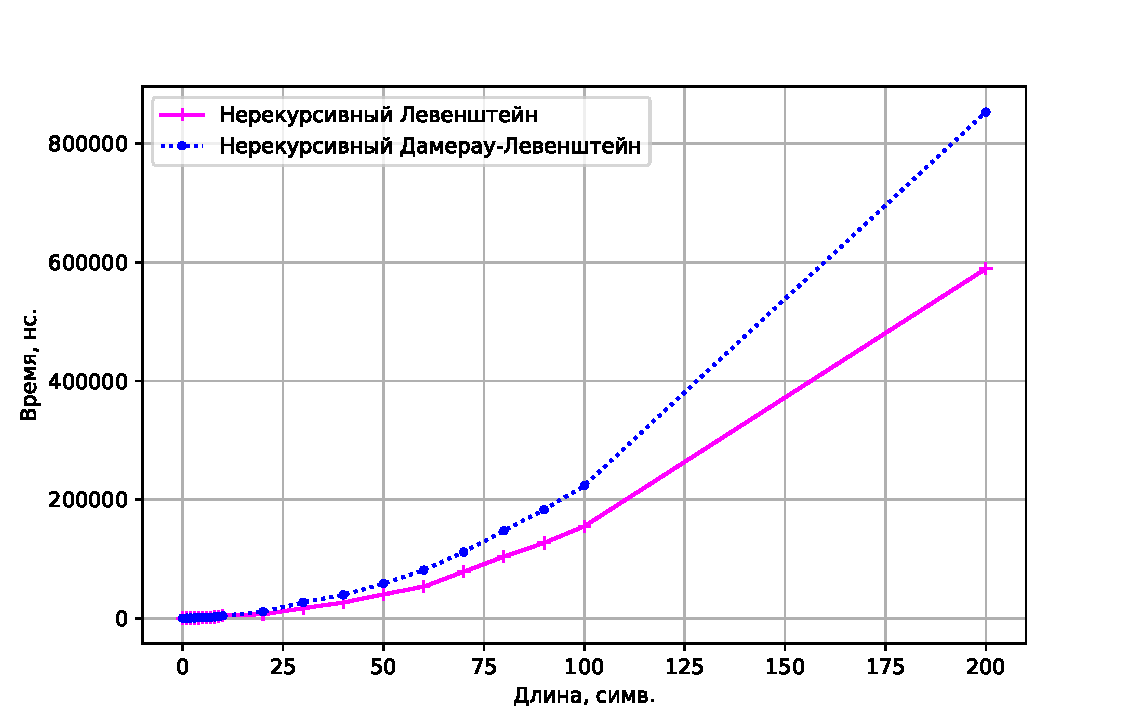
\includegraphics[height=0.4\textheight, page=1]{img/figures.pdf}
	\caption{Сравнение по времени алгоритмов умножения матриц на четных размерах матрицы}
	\label{plt:time_01}
\end{figure}

\begin{figure}[H]
	\centering
	\includegraphics[height=0.4\textheight, page=2]{img/figures.pdf}
	\caption{Сравнение по времени алгоритмов умножения матриц на нечетных размерах матрицы}
	\label{plt:time_02}
\end{figure}

\section*{Вывод}
Исходя из данных, полученных в таблицах \ref{tbl:time_even}--\ref{tbl:time_even}, можно сделать вывод, что лучше всего работает отмизированный алгоритм Винограда.
Стандартный же алгоритм умножения матриц работает 1.6 в раз хуже, чем алгоритм Винограда при четном размере строк и в 1.3 раз хуже при нечетном.

Это обусловлено проведением дополнительных вычислений для крайних строк и cтолбцов. Таким образом, алгоритм Винограда стоит использовать при работе именно с матрицами, размер которых~--- четный.
	\chapter*{Заключение}
\addcontentsline{toc}{chapter}{Заключение}

В ходе исследования было определено, что оптимизированный алгоритм Винограда продемонстрировал лучшую производительность. 
В то же время стандартный метод умножения матриц работает медленнее по сравнению с обеими реализациями алгоритма Винограда. 
Внесенные модификации в оптимизированную реализацию также оказали влияние на ее скорость. 
Кроме того, при использовании алгоритма Винограда с четным размером матриц производительность выше, поскольку нет необходимости в дополнительных вычислениях для крайних строк и столбцов в случае нечетного размера. 
В результате рекомендуется использовать алгоритм Винограда при работе с матрицами четного размера.

Кроме того, реализация алгоритма Штрассена требует больше времени на выполнение из-за дополнительных операций сложения и вычитания матриц.

С учетом теоретических расчетов потребляемой памяти можно сделать вывод о том, что стандартное умножение требует наименьшее количество памяти. 
Однако реализация алгоритма Штрассена требует наибольших затрат памяти из-за необходимости разбивать исходные матрицы на 4 подматрицы при каждом рекурсивном вызове, а также производить дополнительные операции сложения и умножения. 
Оптимизированная реализация алгоритма Винограда также требует больше памяти по сравнению с неоптимизированной из-за использования дополнительных переменных для хранения некоторых предварительных вычислений. 

Цель данной лабораторной работы была достигнута, а именно были исследованы алгоритмы умножения матриц.

В результате выполнения лабораторной работы для достижения этой цели были выполнены следующие задачи:
\begin{enumerate}
    \item описаны следующие алгоритмы умножения матриц:
        \begin{itemize}
            \item стандартный алгоритм умножения;
            \item алгоритм Винограда;
            \item оптимизированный алгоритм Винограда;
            \item алгоритм Штрассена.
        \end{itemize}
    \item релизованы описанные алгоритмы;
    \item дана оценка трудоемкости алгоритмов;
    \item дана оценка потребляемой памяти реализацими алгоритмов;
    \item проведены замеры времени выполнения алгоритмов;
\end{enumerate}


	
	
	\makebibliography
	
	\begin{appendices}
	\chapter{}
	\includelistingpretty
	{merge.cpp} % Имя файла с расширением (файл должен быть расположен в директории inc/lst/)
	{c++} % Язык программирования (необязательный аргумент)
	{Реализация слияния отсортированных подмассивов} % Подпись листинга
	
	\includelistingpretty
	{mergeSort.cpp} % Имя файла с расширением (файл должен быть расположен в директории inc/lst/)
	{c++} % Язык программирования (необязательный аргумент)
	{Реализация алгоритма сортировки слиянием, при использовании 1 потока} % Подпись листинга
	
	\includelistingpretty
	{mergeSortMultiThread.cpp} % Имя файла с расширением (файл должен быть расположен в директории inc/lst/)
	{c++} % Язык программирования (необязательный аргумент)
	{Реализация алгоритма сортировки слиянием, при использовании заданного числа потоков} % Подпись листинга
	
	
	
	
 
\end{appendices}

	
	
\end{document}